% Compile from this directory with: pdflatex InsertionSort.tex
\documentclass[tikz,border=3pt]{standalone}
\usepackage[T1]{fontenc}
\usepackage{helvet}

% #1: horizontal offset; #2: number of boxed elements;
% #3: position of the inserted value (one-based); #4: array values.
\newcommand{\sortarray}[4]{%
    \begin{scope}[xshift=#1]
        \pgfmathtruncatemacro{\boxedcount}{#2}
        \foreach \value [count=\column from 1] in {#4} {
            \node at (\column-0.5,0) {\value};
        }
        \draw[sorted] (0,-0.55) rectangle (\boxedcount,0.55);
        \foreach \column in {1,...,\boxedcount} {
            \draw[sorted] (\column,-0.55) -- (\column,0.55);
        }
        % Draw last so all four edges of the selected cell are red.
        \draw[selected] (#3-1,-0.55) rectangle (#3,0.55);
    \end{scope}%
}

% #1: iteration; #2: insertion position; #3/#4: before/after arrays.
\newcommand{\sortstep}[4]{%
    \begin{scope}[shift={(0,{-1.35*(#1-1)})}]
        \node[anchor=east] at (-0.3,0) {i = #1 :};
        \sortarray{0cm}{#1}{#1+1}{#3}
        \node at (8.6,0) {$\longrightarrow$};
        \sortarray{9.3cm}{#1+1}{#2}{#4}
    \end{scope}%
}

\begin{document}
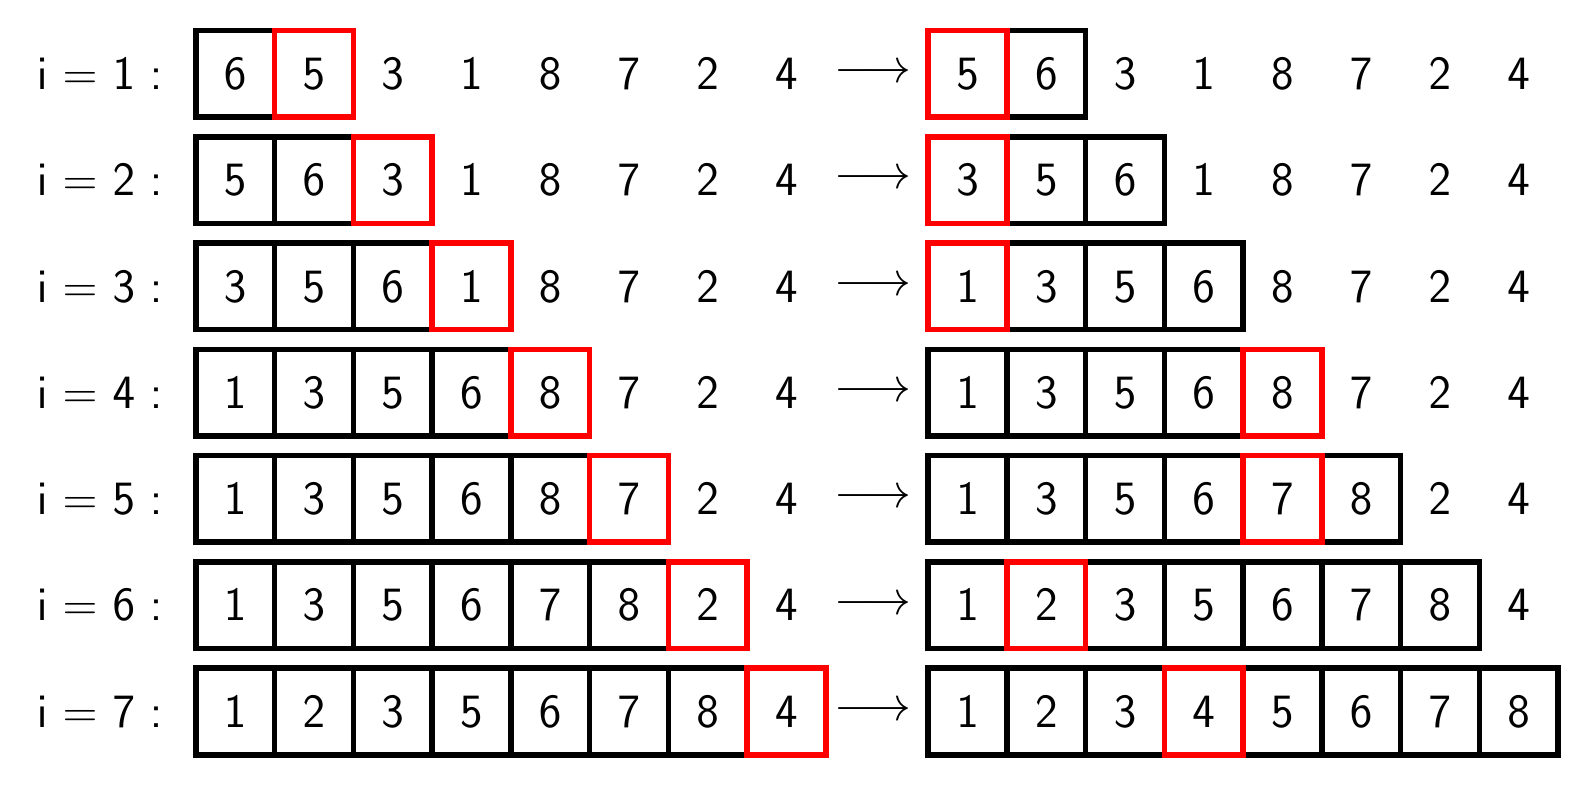
\begin{tikzpicture}[x=1cm,y=1cm,
    font=\sffamily\fontsize{18}{21}\selectfont,
    sorted/.style={black,line width=2pt},
    selected/.style={red,line width=2pt}]
    \sortstep{1}{1}{6,5,3,1,8,7,2,4}{5,6,3,1,8,7,2,4}
    \sortstep{2}{1}{5,6,3,1,8,7,2,4}{3,5,6,1,8,7,2,4}
    \sortstep{3}{1}{3,5,6,1,8,7,2,4}{1,3,5,6,8,7,2,4}
    \sortstep{4}{5}{1,3,5,6,8,7,2,4}{1,3,5,6,8,7,2,4}
    \sortstep{5}{5}{1,3,5,6,8,7,2,4}{1,3,5,6,7,8,2,4}
    \sortstep{6}{2}{1,3,5,6,7,8,2,4}{1,2,3,5,6,7,8,4}
    \sortstep{7}{4}{1,2,3,5,6,7,8,4}{1,2,3,4,5,6,7,8}
\end{tikzpicture}
\end{document}
